\documentclass[a4paper]{article}
\usepackage{times}
\usepackage[utf8]{inputenc}
\usepackage{selinput}
\usepackage{upquote}
\usepackage[margin=2cm, rmargin=4cm, tmargin=3cm]{geometry}
\usepackage{tcolorbox}
\usepackage{xspace}
\usepackage[french]{babel}
\usepackage{url}
\usepackage{hyperref}
\usepackage{fontawesome5}
\usepackage{marginnote}
\usepackage{ulem}
\usepackage{tcolorbox}
\usepackage{graphicx}
%\usepackage[top=Bcm, bottom=Hcm, outer=Ccm, inner=Acm, heightrounded, marginparwidth=Ecm, marginparsep=Dcm]{geometry}


\newtcolorbox{Example}[1]{colback=white,left=20pt,colframe=slideblue,fonttitle=\bfseries,title=#1}
\newtcolorbox{Solutions}[1]{colback=white,left=20pt,colframe=green,fonttitle=\bfseries,title=#1}
\newtcolorbox{Conseils}[1]{colback=white,left=20pt,colframe=slideblue,fonttitle=\bfseries,title=#1}
\newtcolorbox{Warning}[1]{colback=white,left=20pt,colframe=warning,fonttitle=\bfseries,title=#1}

\setlength\parindent{0pt}

  %Exercice environment
  \newcounter{exercice}
  \newenvironment{Exercice}[1][]
  {
  \par
  \stepcounter{exercice}\textbf{Question \arabic{exercice}:} (\faClock \enskip \textit{#1})
  }
  {\bigskip}
  

% Title
\newcommand{\titre}{\begin{center}
  \section*{Algorithmes et Pensée Computationnelle}
\end{center}}
\newcommand{\cours}[1]
{\begin{center} 
  \textit{#1}\\
\end{center}
  }


\newcommand{\exemple}[1]{\newline~\textbf{Exemple :} #1}
%\newcommand{\attention}[1]{\newline\faExclamationTriangle~\textbf{Attention :} #1}

% Documentation url (escape \# in the TP document)
\newcommand{\documentation}[1]{\faBookOpen~Documentation : \href{#1}{#1}}

% Clef API
\newcommand{\apikey}[1]{\faKey~Clé API : \lstinline{#1}}
\newcommand{\apiendpoint}[1]{\faGlobe~Url de base de l'API \href{#1}{#1}}

%Listing Python style
\usepackage{color}
\definecolor{slideblue}{RGB}{33,131,189}
\definecolor{green}{RGB}{0,190,100}
\definecolor{blue}{RGB}{121,142,213}
\definecolor{grey}{RGB}{120,120,120}
\definecolor{warning}{RGB}{235,186,1}

\usepackage{listings}
\lstdefinelanguage{texte}{
    keywordstyle=\color{black},
    numbers=none,
    frame=none,
    literate=
           {é}{{\'e}}1
           {è}{{\`e}}1
           {ê}{{\^e}}1
           {à}{{\`a}}1
           {â}{{\^a}}1
           {ù}{{\`u}}1
           {ü}{{\"u}}1
           {î}{{\^i}}1
           {ï}{{\"i}}1
           {ë}{{\"e}}1
           {Ç}{{\,C}}1
           {ç}{{\,c}}1,
    columns=fullflexible,keepspaces,
	breaklines=true,
	breakatwhitespace=true,
}
\lstset{
    language=Python,
	basicstyle=\bfseries\footnotesize,
	breaklines=true,
	breakatwhitespace=true,
	commentstyle=\color{grey},
	stringstyle=\color{slideblue},
  keywordstyle=\color{slideblue},
	morekeywords={with, as, True, False, Float, join, None, main, argparse, self, sort, __eq__, __add__, __ne__, __radd__, __del__, __ge__, __gt__, split, os, endswith, is_file, scandir, @classmethod},
	deletekeywords={id},
	showspaces=false,
	showstringspaces=false,
	columns=fullflexible,keepspaces,
	literate=
           {é}{{\'e}}1
           {è}{{\`e}}1
           {ê}{{\^e}}1
           {à}{{\`a}}1
           {â}{{\^a}}1
           {ù}{{\`u}}1
           {ü}{{\"u}}1
           {î}{{\^i}}1
           {ï}{{\"i}}1
           {ë}{{\"e}}1
           {Ç}{{\,C}}1
           {ç}{{\,c}}1,
    numbers=left,
}

\newtcbox{\mybox}{nobeforeafter,colframe=white,colback=slideblue,boxrule=0.5pt,arc=1.5pt, boxsep=0pt,left=2pt,right=2pt,top=2pt,bottom=2pt,tcbox raise base}
\newcommand{\projet}{\mybox{\textcolor{white}{\small projet}}\xspace}
\newcommand{\optionnel}{\mybox{\textcolor{white}{\small Optionnel}}\xspace}
\newcommand{\advanced}{\mybox{\textcolor{white}{\small Pour aller plus loin}}\xspace}
\newcommand{\auto}{\mybox{\textcolor{white}{\small Auto-évaluation}}\xspace}


\usepackage{environ}
\newif\ifShowSolution
\NewEnviron{solution}{
  \ifShowSolution
	\begin{Solutions}{\faTerminal \enskip Solution}
		\BODY
	\end{Solutions}
  \fi}


  \usepackage{environ}
  \newif\ifShowConseil
  \NewEnviron{conseil}{
    \ifShowConseil
    \begin{Conseils}{\faLightbulb \quad Conseil}
      \BODY
    \end{Conseils}

    \fi}

    \usepackage{environ}
  \newif\ifShowWarning
  \NewEnviron{attention}{
    \ifShowWarning
    \begin{Warning}{\faExclamationTriangle \quad Attention}
      \BODY
    \end{Warning}

    \fi}
  

%\newcommand{\Conseil}[1]{\ifShowIndice\ \newline\faLightbulb[regular]~#1\fi}



\usepackage{minted}
\usepackage{array}
\newcolumntype{C}[1]{>{\centering\let\newline\\\arraybackslash\hspace{0pt}}m{#1}}

\begin{document}

% Change the following values to true to show the solutions or/and the hints
\ShowSolutiontrue
\ShowConseiltrue
\titre
\cours{Semaine 6}
\cours{Algorithmes de recherche}



\begin{enumerate}
    \item Recherche séquentielle
    \item Recherche binaire
    \item Arbres de recherche binaire\\
\end{enumerate}

Le but de cette séance est de se familiariser avec les algorithmes de recherches.\\

\section{Recherche séquentielle (ou recherche linéaire)}

\subsection{Définition}

Une recherche \textbf{linéaire} (ou \textbf{séquentielle}) est une méthode permettant de trouver un élément dans une liste, un tableau ou un dictionnaire. Elle vérifie un à un chaque élément de gauche à droite jusqu'à ce qu'une correspondance soit trouvée ou que toute la liste ait été recherchée.\\

Si l'élément recherché est trouvé, l'algorithme \textbf{renvoie l'index}, c'est-à-dire la position, de l'élément dans la liste donnée. \\

Sa complexité dans le pire des cas est de \textbf{O(n)}, la longueur de la liste, et dans le meilleur des cas de \textbf{O(1)}, lorsque l'élément se trouve en première position. Dans la pratique, l'algorithme de recherche séquentielle n'est pas souvent utilisé en vue de sa complexité élevée et des alternatives de recherche plus efficaces comme la recherche binaire.\\\

\subsection{Exercices}

\begin{Exercice}[5 minutes] language : \textbf{Python}\\

A partir des éléments ci-dessous, écrivez une fonction qui cherche \lstinline{x} dans la liste.\\La fonction doit retourner l'index de l'élément correspondant de la liste si \lstinline{x} est dans la liste et "-1" si \lstinline{x} n'est pas dans la liste (avec \lstinline{x = 100})\\

\textbf{Python :}
\begin{lstlisting}{python}
    def plus_proche_sequentielle(liste, x):
        #complètez ici
        
    
    
    L = [3,55,6,8,3,5,56,33,6,5,3,2,99,53,532,75,21,963,100,445,56,56,24]
    x = 100
    
    plus_proche_sequentielle(L, x)
        
    %%time #Permet d'afficher le temps d'exécution de l'algorithme 
    print(plus_proche_sequentielle(L, x))
    
\end{lstlisting}

\begin{conseil}
    Définissez votre fonction de recherche linéaire en utilisant une boucle \lstinline{for} ou une boucle \lstinline{while}.\\\\
    Attention: la fonction doit retourné l'index de la valeur et non pas la valeur. Pour cela, veillez à utiliser \lstinline{range(len(list))} avec la boucle \lstinline{for} et une incrémentation \lstinline{"i = i+1"} avec la boucle \lstinline{while}.\\\\
    La fonction \lstinline{print()} vous permet d'afficher l'index lorsqu'il a été trouvé et un autre message le cas échéant. 
\end{conseil}
    
\begin{solution}
\textbf{Python :}
    \lstinputlisting{solutions/question1.py}
    
\end{solution}

\end{Exercice}

\begin{Exercice}[10 minutes] language : \textbf{Python}\\

Considérez une liste d’entiers non triée \lstinline{L} ainsi qu’un entier \lstinline{e}. Écrivez un programme qui retourne l'élément de la liste \lstinline{L} dont la valeur est la plus proche de \lstinline{e} en utilisant une recherche séquentielle.\\\\
Exemple :\\
L = [16, 2, 25, 8, 12, 31, 2, 56, 58, 63]\\
e = 50\\
Résultat attendu : 56\\
\textbf{Python :}
\begin{lstlisting}{python}
    #Definition de la fonction ayant pour argument une liste et un nombre 
    def plus_proche_sequentielle(list,n):
        diff = None #Initialisation de la variable pour la différence
        resultat = None #Initialisation de la variable pour le résultat
    
        #Complètez ici
        
    #Déclaration de la liste et de la variable e
    L = [16, 2, 25, 8, 12, 31, 2, 56, 58, 63] 
    e = 50

    #Exécution de la fonction
    plus_proche_sequentielle(L,e)
    
    %%time 
    print(plus_proche_sequentielle(L,e))

\end{lstlisting}

    \begin{conseil}
        Complétez la fonction \lstinline{plus_proche_sequentielle} et exécutez le code.\\\\
        Veillez à utiliser les valeurs absolues pour comparer les différences, la plus petite pouvant être positive ou négative. La fonction \lstinline{abs()} retourne la valeur absolue. Exemple : \lstinline{abs(3-10) retourne 7}.\\\\
        Étant donné que la liste est \textbf{non triée}, l'algorithme doit obligatoirement la parcourir intégralement.\\\\
        L'algorithme doit calculer la différence entre \lstinline{e} et chaque élément de la liste \lstinline{L} en gardant toujours la plus petite différence trouvée. À la fin, il retourne l'élément de la liste correspondant à la plus petite différence.  
    \end{conseil}
    
    \begin{solution}
    \textbf{Python :}
        \lstinputlisting{solutions/question2.py}
        
    \end{solution}
    
\end{Exercice}

\begin{Exercice}[5 minutes] language : \textbf{Python}\\

    Considérez une \textbf{liste d’entiers triés} \lstinline{L} ainsi qu’un entier \lstinline{e}. Écrivez un programme qui retourne l'index de l'élément \lstinline{e} de la liste \lstinline{L} en utilisant une recherche séquentielle. Si \lstinline{e} n’est pas dans \lstinline{L}, retournez -1.\\\\
    
    Exemple:\\
    L = [1231321,3213125,3284016,4729273,5492710]\\
    e = 3284016\\
    Résultat attendu: 2\\
  
\begin{lstlisting}{python}
    def recherche_lineaire(L,e):
        for i in L: #Ici, i correspond à la valeur et non l'index.
        #complètez ici 
        
    L = [1231321,3213125,3284016,4729273,5492710]
    e = 3284016
    recherche_lineaire(L,e)
    
    %%time
    print(recherche_lineaire(L,e))
\end{lstlisting}

    \begin{conseil}
        Une liste triée permet une recherche plus efficace à l'aide d'un algorithme plus simple.\\\\
        Veillez à retourner l'index de la valeur dans la liste. La fonction \lstinline{index()} retourne l'index d'un élément au sein d'une liste.\\Exemple et syntaxe: \lstinline{lst.index(i)} va indiqué la position de l'élément \lstinline{i} dans la liste \lstinline{lst}.
    \end{conseil}


    \begin{solution}
        \textbf{Python :}
        \lstinputlisting{solutions/question3.py}
    \end{solution}
\end{Exercice}

\newpage
\section{Recherche binaire}

\subsection{Définition}

Le but de la recherche binaire est de trouver l'élément \lstinline{x} plus rapidement. Pour cela, il est nécessaire d'utiliser \textbf{une liste d'éléments triée}.\\

La complexité de l'algorithme de recherche binaire est \lstinline{O(log n)}. Cependant, il ne faut pas oublier le coût lié à l'obtention d'une liste triée à partir d'une liste non triée.\\

L'algorithme de recherche binaire divise l'intervalle de recherche par deux à chaque coup jusqu'à ce qu'il trouve l'élément \lstinline{x} ou que l'intervalle soit vide.\\

Ainsi, si \lstinline{x} est plus petit que l'élément du milieu, l'algorithme va choisir la moitié de gauche comme intervalle de recherche et ainsi de suite. Si \lstinline{x} est plus grand que l'élément du milieu la recherche va se faire dans la moitié droite de l'intervalle.\\

La recherche binaire regarde les comparaisons d'ordre, alors que la recherche séquentielle regarde les comparaisons d'égalité pour trouver x.\\

\subsection{La récursivité}

Une fonction récursive est une fonction qui s'appelle elle-même pendant son exécution. Vous trouverez ci-dessous un exemple de fonction récursive utilisée pour le calcul factoriel.

\begin{lstlisting}{python}
    def factoriel(n):
        if n == 1:
            return n
        else:
            return n * factoriel(n - 1)
            
    factorielle(4)
    #La fonction calcul 4 factoriel et retourne le résultat 
    #Rappel : 4! = 4 x 3 x 2 x 1 = 24
\end{lstlisting}

Les fonctions récursives sont courantes en informatique car elles permettent aux programmeurs d'écrire des programmes efficaces en utilisant une quantité minimale de code. L'inconvénient est qu'elles peuvent provoquer des boucles infinies et d'autres résultats inattendus si elles ne sont pas écrites correctement. Si la fonction n'inclut pas les cas appropriés pour arrêter l'exécution, la récursivité se répétera à l'infini, provoquant le plantage du programme ou, pire encore, l'arrêt de tout le système informatique.\\
   
\subsection{Exercices}

\begin{Exercice}[20 minutes] language : \textbf{Python}\\

A partir de la liste d'éléments \textbf{triée} ci-dessous, écrivez premièrement \textbf{une fonction récursive} puis \textbf{une fonction itérative} qui cherche \lstinline{x} dans la liste. La fonction doit retourner \textbf{l'index} de l'élément correspondant de la liste si \lstinline{x} est dans la liste et \lstinline{-1} dans le cas contraire.\\
Ici, \lstinline{x = 5}.\\

\begin{lstlisting}{python}
    #Version récursive
    
    def recherche_binaire_recursive(liste,s,r,x):
        #complètez ici 
    
    L=[1,3,4,5,7,8,9,15]
    s = 0
    r = len(L)
    x = 5
    recherche_binaire_recursive(L,s, r, x)
 
    %%time
    print(recherche_binaire_recursive(L,s, r, x))

    
    ##################################################

    #Version itérative
    
    def recherche_binaire_iterative(liste,s,r,x):
      #complètez ici
      
    L = [1,3,4,5,7,8,9,15]
    s = 0
    r = len(L)-1
    x = 7
    recherche_binaire_iterative(L,s, r, x)
    
    %%time
    print(recherche_binaire_iterative(L,s, r, x))
\end{lstlisting}

    \begin{conseil}
        Complétez la fonction récursive \lstinline{recherche_binaire_recursive} et la fonction itérative \lstinline{recherche_binaire_iterative}.\\\\
        Détails sur les arguments de la fonction:\\
        \lstinline{L} : La liste dans laquelle nous effectuons la recherche\\
        \lstinline{s} : Le premier élément de la liste (index [0])\\
        \lstinline{r} : Le dernier élément de la liste (index [longueur de la liste -1])\\
        \lstinline{x} : La valeur recherchée.\\\\

        Ainsi, à chaque itération, vos fonction vont modifier les valeurs de base données en argument pour resserrer l'intervalle jusqu'à trouver la valeur recherchée.\\        
        Pour définir le milieu d'un intervalle qui contient un nombre pair ou impair d'éléments, utilisez la fonction \lstinline{int()}. Exemple:\\
        liste1 = [1,2,3,4,5]
        s = 0 \quad r = len(liste1)
        Calcul du milieu de l'intervalle:\\
        - \lstinline{(s+r)/2) = (0+5)/2 = 2.5 #Pas de correspondance}\\
        - \lstinline{int((s+r)/2) = int((0+5)/2) = int(2.5) = 2 #Arrondi vers le bas}\\\\
        
        Pour la version itérative, il est conseillé d'utiliser une boucle \lstinline{while}.

    \end{conseil}

    \begin{solution}
        \textbf{Python :}
        \lstinputlisting{solutions/question4-1.py}
    \end{solution}
    \begin{solution}
        \textbf{Python :}
        \lstinputlisting{solutions/question4-2.py}
    \end{solution}

\end{Exercice}


\begin{Exercice}[15 minutes] language : \textbf{Python}\\

Considérez une liste d’entiers \textbf{triés} \lstinline{L} ainsi qu’un entier \lstinline{e}. Écrivez un programme qui retourne l'élément de la liste \lstinline{L} le plus proche de \lstinline{e} en utilisant une recherche binaire.\\

On vous donne une liste d’entiers \textbf{triés} \lstinline{L} ainsi qu’un entier \lstinline{e}. Écrivez un programme retournant la valeur dans \lstinline{L} la plus proche de \lstinline{e} en utilisant une recherche binaire (binary search).\\

Résultat attendu : 56\\

    \begin{lstlisting}{python}
    def plus_proche_binaire(liste,n):
        #complètez ici
        
        
    L = [1, 2, 5, 8, 12, 16, 24, 56, 58, 63]  
    e = 41
    plus_proche_binaire(L,e)
    
    %%time
    print(plus_proche_binaire(L,e))
    \end{lstlisting}

\begin{conseil}
    Veillez à définir des variables \lstinline{min} et \lstinline{max} délimitant l'intervalle de recherche et une variable booléenne \lstinline{found} initialisée \lstinline{false} et qui devient \lstinline{true} lorsque l'algorithme a trouvé la valeur la plus proche de \lstinline{e}. 
    
\end{conseil}

    \begin{solution}
        \textbf{Python :}
        \lstinputlisting{solutions/question5.py}
    \end{solution}

\end{Exercice}

\begin{Exercice}[10 minutes] language : \textbf{Python}\\

Considérez une liste d’entiers triés \lstinline{L} ainsi qu’un entier \lstinline{e}. Écrivez un programme qui retourne l'index de l'élément \lstinline{e} de la liste L en utilisant une recherche binaire. Si \lstinline{e} n’est pas dans \lstinline{L}, retournez \lstinline{-1}.\\\\

Exemple:\\

    L = [1231321,3213125,3284016,4729273,5492710] \\

    e = 3284016\\

Résultat attendu: 2\\

    \begin{lstlisting}{python}
    def recherche_binaire(liste,e):
        first = 0 
        last = len(L)-1
        
        #complètez ici
    
    
    L = [1231321,3213125,3284016,4729273,5492710]
    e = 3284016
    recherche_binaire(L,e)
    
    %%time
    print(recherche_binaire(L,e))
    \end{lstlisting}

\begin{conseil}
    Inspirez-vous des exercices et des conseils précédents. 
\end{conseil}

    \begin{solution}
        \textbf{Python :}
        \lstinputlisting{solutions/question6.py}
    \end{solution}

\end{Exercice}


\begin{Exercice}[10 minutes] language : \textbf{Python}\\
    
    \textbf{Matrice en Python}

    Considérez une matrice ordonnée m et un élément l.\\\\
    
    Une matrice ordonnée répond aux critères suivants :\\
     \lstinline{[i][j]<=m[i+1][j]} (une ligne va du plus petit au plus grand)\\
     \lstinline{[i][j]<=m[i][j+1]} (une colonne va du plus petit au plus grand)\\\\
 
    
    Écrivez un algorithme qui retourne la position de l’élément l dans m. Si l n’est pas présent dans m alors il faut retourner (-1, -1)\\\\
    
    Exemple 1: si m=[[1,2,3,4],[4,5,7,8],[5,6,8,10],[6,7,9,11]] et que l=7. Nous souhaitons avoir la réponse (1,2) OU (3,1) (l’une des deux, pas besoin de retourner les deux résultats).\\\\
    
    Exemple 2: si m=[[1,2],[3,4]] et que l=7. Nous souhaitons avoir la réponse (-1,-1) car 7 n’est pas dans la matrix m.\\


    \begin{lstlisting}{python}
    def recherche_matricielle(m,l):
        #complètez ici
    
    
    m=[[1,2,3,4],[4,5,7,8],[5,6,8,10],[6,7,9,11]]
    l=7
    recherche_matricielle(m,l)
    \end{lstlisting}

    \begin{conseil}
    Pour cet exercice il est nécessaire d'utiliser une double boucle \lstinline{for}, c'est-à-dire: une boucle \lstinline{for} dans une boucle \lstinline{for}. Cela permet de parcourir tout les éléments d'un tableau à deux dimensions à l'exemple d'une matrice. 
    \end{conseil}

    \begin{solution}
        \textbf{Python :}
        \lstinputlisting{solutions/question7.py}
    \end{solution}

\end{Exercice}

\newpage
\section{Arbre de recherche binaire}
\subsection{Définition}

Un arbre de recherche binaire est une structure de donnée au même titre que les listes, tuples, dictionnaires, etc. Leur particularité est qu'au lieu d'ordonner les éléments les uns à la suite des autres, les arbres de recherche binaire enregistrent les valeurs de manière relationnelle.\\

En effet, l'arbre est divisé en branches qui peuvent elles-même contenir deux branches (enfants) et ainsi de suite. Lorsqu'une branche n'a pas de branches subséquentes (enfants), on parle de feuille.\\

Les branches peuvent donc contenir de 0 à 2 autres branches. On parle alors de la branche à gauche et de celle à droite. La branche de gauche est forcément plus petite que la branche parente et celle de droite est forcément plus grande.\\

De cette façon, on garantit que l'arbre est toujours ordonné même en rajoutant ou en retirant des éléments\\

\begin{figure}[h]
    \centering
    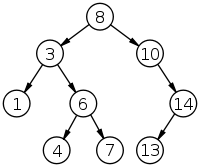
\includegraphics[width=0.32\textwidth]{img/binary-search-tree.png}
    \caption{Exemple d'arbre binaire}
\end{figure}

\subsection{Exercices}

\begin{Exercice}[15 minutes] language : \textbf{Python}\\
    
    Dans l'exercice suivant nous vous donnons un arbre binaire avec les mêmes valeur que le schéma précédent et dont la racine est la variable root.\\

    Ecrivez une fonction qui retourne \lstinline{True} si la valeur valeur est dans l'arbre et \lstinline{False}, sinon. Vous pouvez utiliser la variable value pour afficher la valeur d'une node et les variables \lstinline{left} et \lstinline{right} sur les \lstinline{nodes} pour accèder aux branches enfantes, \lstinline{node.value}, \lstinline{node.left} et \lstinline{node.right}.\\\\
    Complétez la fonction \lstinline{recherche_arbre}.\\
    \begin{lstlisting}{python}
    import sys
    import traceback
    from Arbre import Arbre
    
    def recherche_arbre(node, value):
        # Complétez ici
        
    
    
    def handle_error(): #Fonction appelée dans le bloc "except" qui gère les erreurs
        _, _, tb = sys.exc_info()
        traceback.print_tb(tb) 
        tb_info = traceback.extract_tb(tb)
        filename, line, func, text = tb_info[-1]
        print('Une erreur s\'est produite sur la ligne {} dans la déclaration {}'.format(line, text))
    
    try: #"try" permet de tester le code pour détecter les erreurs.
    
        tree = Arbre(8, 3, 1, 6, 4, 7, 10, 14, 13)
        root = tree.root
        assert recherche_arbre(root, 4) == True # devrait trouver
        assert recherche_arbre(root, 7) == True # devrait trouver
        assert recherche_arbre(root, 18) == False # ne devrait pas trouver
        assert recherche_arbre(root, 21) == False # ne devrait pas trouver
    
        print("Bonne réponse avec le premier arbre")
    except AssertionError: #"except" permet de gérer l'erreur
        handle_error()
        print("Mauvaise réponse")
        
    try:
        tree = Arbre(1, 3, 9, 6, 14, -17, 110, 124, 13, -1, 9, 1, 40, -98, 120, 23)
        root = tree.root
        assert recherche_arbre(root, 14) == True # devrait trouver
        assert recherche_arbre(root, 110) == True # devrait trouver
        assert recherche_arbre(root, 39) == False # ne devrait pas trouver
        assert recherche_arbre(root, 18) == False # ne devrait pas trouver
        print("Bonne réponse avec le deuxième arbre")
    except AssertionError as err:
        handle_error()
        print("Mauvaise réponse")

    \end{lstlisting}

    \begin{conseil}
    Indice: Utilisez une fonction récursive.
    \end{conseil}

    \begin{solution}
        \textbf{Python :}
        \lstinputlisting{solutions/question8.py}
    \end{solution}

\end{Exercice}



\end{document}